

\documentclass[]{article}
%\usepackage[latin1]{inputenc}
\usepackage[utf8]{inputenc}
% Esto es para que el LaTeX sepa que el texto está en español:
%\usepackage[spanish]{babel}

% Paquetes de la AMS:
\usepackage{amsmath, amsthm, amsfonts}
\usepackage{graphicx}

%opening
\title{Trabajo Práctico 1}
\author{Jairo Jiménez \\
	Sergio De Raco}

\begin{document}

\maketitle


\section*{Objetivo}
El objetivo del presente trabajo es analizar las característcas en las cuáles el algoritmo J48 es robusto. El algoritmo será aplicado sobre la base de datos Latinobarómetro, la cual es una encuesta de percepción política, democrática y social de latinoamérica. Para poder observar las cualidades y deficiencias del algoritmo, este será sometido a diferentes tipos de pruebas para analizar su comportamiento.

\section*{Alcance}


\section*{Resultados esperados}

\section*{Metodología}

\section{Sobreajuste y poda}

El mejor ajuste del árbol se da cuando la confianza es de 0.1, después de este valor, empieza el sobreajuste del árbol, pues este deja baja la capacidad de pronosticar las nuevas instancias de manera correcta\\
A medida que aumenta la confianza, aumentan el tamaño y el número de hojas

%\begin{figure}
%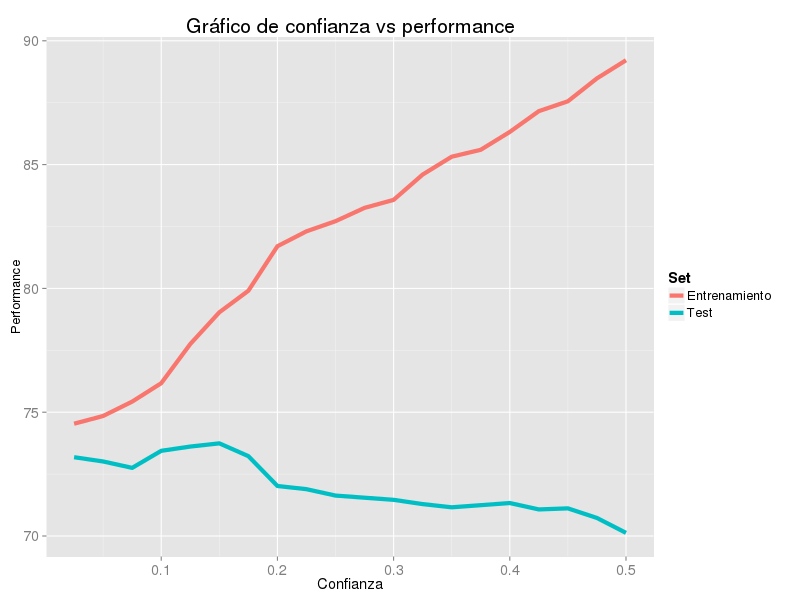
\includegraphics[width=0.8\linewidth,height=0.4\textheight]{Punto_1_Confianza_VS_ajuste}
%\caption[Confianza vs ajuste]{Confianza vs Ajuste}
%\label{P1ConfVSAjus}
%\end{figure}

\begin{figure}
	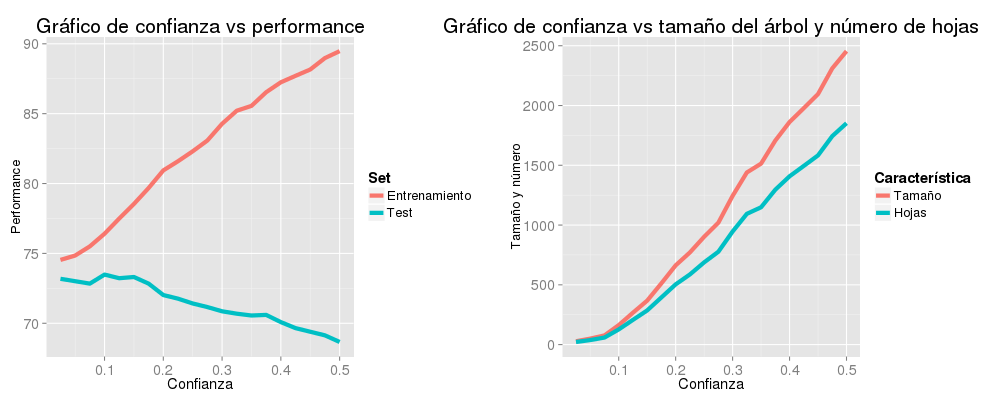
\includegraphics[scale = 0.2]{Punto_1_Graficos_Mezclados}
	\caption[Confianza vs ajuste]{Gráficos de confianza}
	\label{P1Conf}
\end{figure}
%
%
%\begin{figure}
%	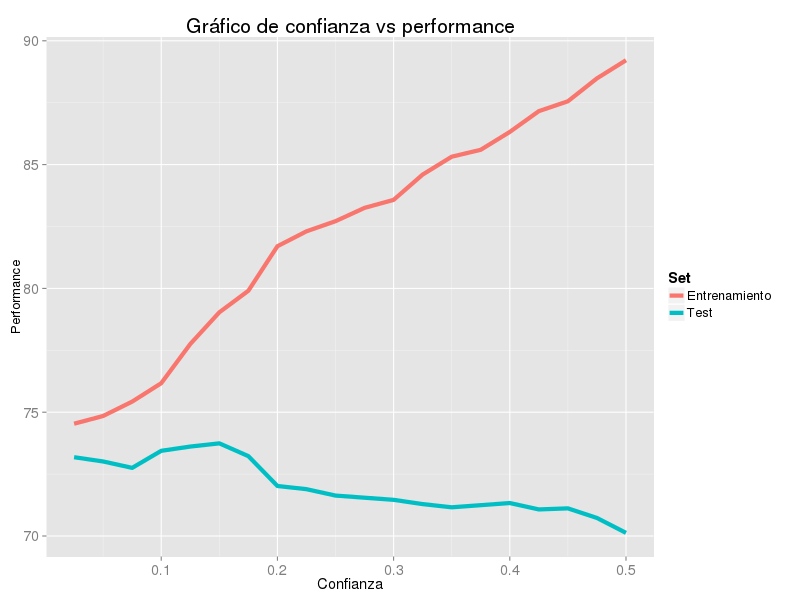
\includegraphics[scale = 0.4]{Punto_1_Confianza_VS_ajuste}
%	\caption[Confianza vs ajuste]{Confianza vs Ajuste}
%	\label{P1ConfVSAjus}
%\end{figure}

%\begin{figure}
%	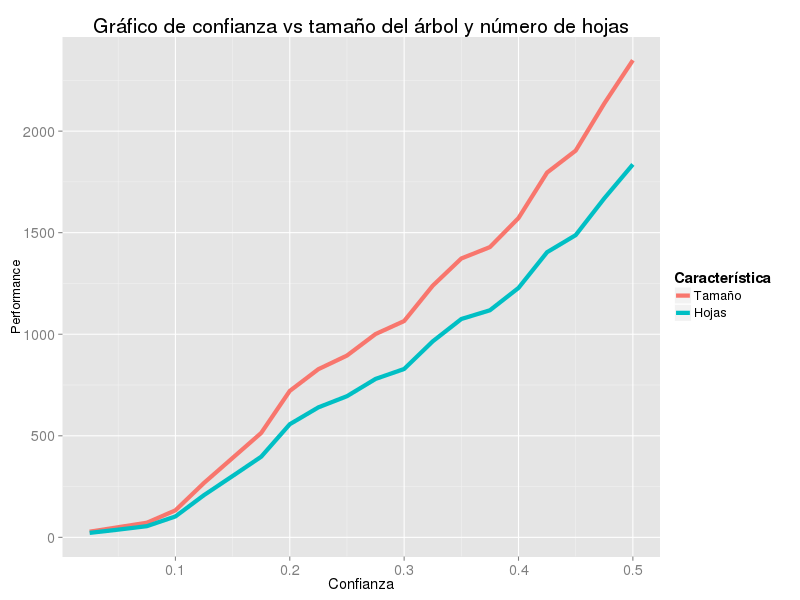
\includegraphics[scale = 0.4]{Punto_1_Confianza_VS_tamano}
%	\caption[Confianza vs ajuste]{Confianza vs Tamaño}
%	\label{P1ConfVSTamano}
%\end{figure}





\section{Tratamiento de datos faltantes}
Para el análisis de datos faltantes, el algoritmo se sometió a 3 diferentes tipos de faltantes sobre el conjunto de datos. Primero se anaklizó el efecto de los datos faltantes sobre una sola columna, luego sobre varias columnas pero solamente induciendo un faltante por fila y por último sobre varias columnas pero induciendo varios faltantes por fila. En los 3 casos, la cantidad de datos faltantes fue aumentando de 0 a 85\%

\subsection{Sobre una sola variable}
En el caso de una variable, se seleccionó como candidata la variable que separa mejor el árbol. A esta variable se le agregaron faltantes desde 0 a 85\%

\subsubsection{Imputación sin tener en cuenta la clase}

\subsubsection{Imputación teniendo en cuenta la clase}

\subsection{Sobre varias variables con un único faltante por fila}
En este caso, se agregaron datos faltantes de manera aleatoria a las columnas, pero tengiendo en cuenta que solamente se admite un valor faltante por fila en el conjunto de datos. 

\subsubsection{Imputación sin tener en cuenta la clase}

\subsubsection{Imputación teniendo en cuenta la clase}

\subsection{Sobre varias variables con múltiples faltantes por fila}
Para el último análisis, se agregaron datos faltantes sobre el total de entradas de el conjunto de datos (total de filas por total de columnas).

\subsubsection{Imputación sin tener en cuenta la clase}

\subsubsection{Imputación teniendo en cuenta la clase}

\section{Tolerancia al ruido}
En esta parte, se genero entre 0 y 35\% de ruido sobre la clase. 

\section{Discretización de atributos numéricos}

\subsection{Sobre variables con poco poder discriminativo}

\subsection{Sobre variables con mucho poder discriminativo}

\section*{Conclusiones}

\section*{Trabajo futuro}

\bibliography{Bibliografia.bib}

\section*{Referencias}

\end{document}
